\section{W11: Outsourcing, Procurement and Contracts}

\textbf{1. Outsourcing}
\textbf{1.1. Onshoring}: relocating activities inside national borders to access target benefits.
\textbf{1.2. Nearshoring}: activities relocated to another country with close proximity e.g. New Zealand, Indonesia
\textbf{1.3. Offshoring}: activities relocated to another country irrelevant of geographical location and timezones.
\textbf{2. The Procurement Management Process.}
    \textbf{2.1. Plan Procurements.}
    \textbf{2.2. Sourcing Procurements.}
        \textbf{2.2.1. Request for x (RFx).}
            \textbf{2.2.1.1. Bid.}
            \textbf{2.2.1.2. Information.}
            \textbf{2.2.1.3. Proposal.}
            \textbf{2.2.1.4. Quotation.}
            \textbf{2.2.1.5. Tender.}
        \textbf{2.2.2. Statement of Work}: description of work required.
        \textbf{2.2.3. Evaluation Processes.}
    \textbf{2.3. Managing Procurements.}
        \textbf{2.3.1. Renewing/Closing Procurements.}
\textbf{3. Fixed Price contracts}: higher risk for seller, lower risk for buyer.
\textbf{4. Time \& Material contracts}: higher risk for buyer, lower risk for seller.
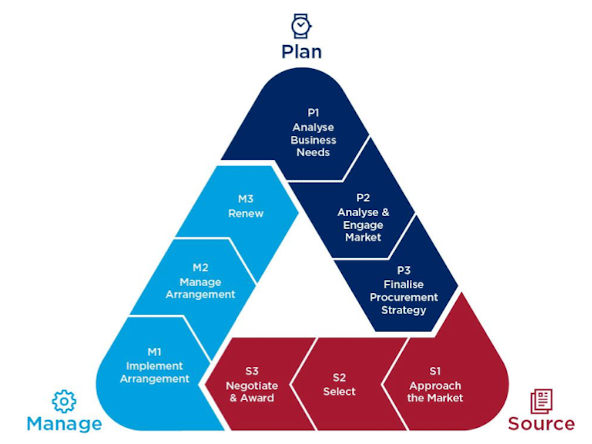
\includegraphics[width=\linewidth]{figs/SCR-20240606-tfgb.png}
